\documentclass[12pt]{article}
\usepackage{wkrpt}
\begin{document}

\title{An Analysis of Using Global Scoped Style Sheets and Atomic Scoped Style Sheets in the Context of Styling Component Based Applications}
{
	Yahoo!\\
	Sunnyvale, CA
}
{
	Aditya Sridhar\\
	3B Software Engineering\\
	Student ID 20539123\\
	User ID a3sridha\\
	September 8, 2016
}


\letter{An Analysis of Using Global Scoped Style Sheets and Atomic Scoped Style Sheets in the Context of Styling Component Based Applications}{3B}{Yahoo!}{Mail Front-end}
{
	\noindent
	Aditya Sridhar\\
	201 Lester Street\\
	Waterloo, ON N2L 3G1
}
{
	Description of your co-op position. This should be about three sentences
}
{
	Description of report and how it related to co-op position.
}
{
	Acknowledgements
}
{
	Aditya Sridhar, 20539123
}


\tocsection{Executive Summary}
EXECUTIVE SUMMARY
\newpage

% para 1: The next generation of Yahoo Mail is built on ReactJS. ReactJS is used to build component-based web application. The idea is that the component is a single unit of the UI and deals with all that is assocciation with that unit(check dan hood ...) This report analyses the use of Atomic CSS (component-scoped) and global scoped CSS

% para 2: A more traditional approach


\toc
% \lof
% \lot


\pagenumbering{arabic}
\section{Introduction}
\subsection{Background Information}

% TODO: state that 2nd para is global CSS and define atomic CSS ??? or do that in first page of BODY

Yahoo! is an internet technology company and is recognized as one of the pioneers of the early-internet era. Yahoo! Mail is a web-based email service owned by Yahoo! with hundreds of millions of users worldwide. The next generation of Yahoo! Mail web client is currently being developed and is built using the ReactJS framework. ReactJS is a component-based JavaScript library used for building user interfaces. The idea behind a component-based framework is that a complex user interface should be broken down into multiple components. Each component should follow the Single Responsibility Principle (SRP), which implies that it should be responsible for single part of the user interface.

Traditionally the development of webpages was based on the principle of Separation of Concerns (SoC) which advocates breaking a problem into different concerns and using a resource to address a particular concern. In the context of web pages, the structure, presentation and behaviour layers were identified as separate concerns with Hyper Text Markup Language (HTML) defining the structure of a web page, Cascading Style Sheets (CSS) defining the content presentation styles and JavaScript (JS) defining how the web page behaves with user interaction. Hence CSS aids in separating web page presentation from web page content.

% Table: separation of concerns web page

\subsection{Introduction to the Issue}
CSS is a collection of rules, each rule containing one or more selectors and a block of styles. These rules are written in style sheets which are then packaged in the main project. A selector is used to identify a particular HTML element in the web page content and the styles specified in the rule are applied to that particular HTML element. The following figure better elaborates ... 

% Figure: <div>This is my web page</div> div { background-color: red };

% TODO: should this be moved to problem description?


% TODO: define different scopes and say how component scope is related to atomic scope

This report compares global-scoped style sheets with component-scoped style sheets in the context of styling component-based projects. It first provides some additional information about the issue and lists a set of design constraints and the evaluation criteria. It identifies the benefits and pitfalls of each accepted solution. The report uses AHP to perform quantitative analysis of the alternatives against a set of evaluation criteria. The report then concludes by identifying the best solution and provides some recommendations.


\section{Problem Specifications}
\subsection{Problem Description}
CSS is an important component of the front-end toolkit. Since the internet is composed of billions of web pages, CSS is being used on a regular basis to govern the look and feel of web pages. One of the main concerns of using CSS is maintainability. CSS is easy to maintain when the web pages have less content, but as the size of the project increases, the maintainability of style sheets decreases. High maintainability implies that a developer can modify a particular rule without worrying about it adversely impacting other rules. Low maintainability hampers the scalability of a project from a design standpoint and significantly affects the developers in the team.

% #TODO: Either insert specificity table or figure comparing how higher specificity of style leads to overrriding thing and explain

As mentioned earlier, a CSS selector targets a particular HTML element in the web page content and the styles linked to the selector is applied to element it targets. As the content of the web page grows, CSS selectors are more specific and descriptive to target a particular element in the web page. This is termed as selector specificity. If two selectors target the same element in the web page content, the selector with higher specificity tends to override the selector with lower specificity. The style sheet containing selectors with high specificity makes it harder for an existing style to be overriden by a new style. Hence low specificity leads to high maintainability.

\begin{figure}[h]
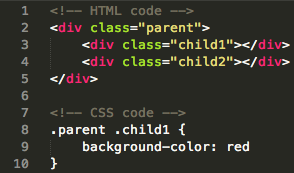
\includegraphics[scale=0.7]{descendent-selector}
\centering
\caption{Example of styling using context-based selectors}
\end{figure}

At times, a developer might want to match a web page element that is a descendent of another web page element. For example in Figure 2.1 the \textit{<div>} element whose class name is \textit{child1} is a descendent of the \textit{<div>} element whose class name is \textit{parent}. The CSS selector \textit{.parent .child1} is an example of a context-based selector. It is targeting the element with class name as \textit{child1} that is a descendent of the element with class name as \textit{parent}. This means that the descendent element is being styled in the context of its parent, and that the rule is redundant outside of this context. This will ultimately lead to more rules being added to the style sheet if the requirement to style the same element outside of the context arises.




% As the number of rules in a style sheet increases, the maintainability decreases. Hence making the styles reusable makes the stylesheets more maintainable. ... Intutive thing ... 


% what is context based styling and descendent selectors and how does it affect maintainablility



% how decoupling .... makes.... 
% why is maintainablity affected
% why context based styling affects maintainabliity..


% In problem description mainly talk about maintainability, and talk about how disadvantages of global CSS leads to maintainability issues. Also introduce topics like contextual selectors



% TODO: explain different types of selectors, explain contextual styling

% IMPORTANT POINT: reducing the scope improves maintainability significantly

\subsection{Design Constraints}
A solution should adhere to the following design constraints, in order to be deemed as an accepted solution:
% Design constraints: 1) If change occurs, should not be applied to every element 3) Ability to style using classes. Refer to https://vineetgupta22.wordpress.com/2011/07/09/inline-vs-internal-vs-external-css/


\subsection{Design Criteria}
The following evaluation criteria are used to compare the two accepted solutions:
\begin{enumerate}

	\item \textbf{Usage of context-based styling should be minimized}: The accepted solution should limit the usage of contextual styling as this demotes reusability and portability of styles. This ultimately makes style sheets hard to maintain.
	% Note: this can be done by limiting the use of descendent selectors. say in global approach this could be kept in mind but hard to enforce as projects grow. In atomic approach this never happens

	\item \textbf{Low specificity of styles}: Low CSS specificity enables the developer to override a CSS rule when requirements change. This makes the style sheets more maintainable.

	\item \textbf{Changes should be intuitive}: The accepted solution should be intuitive and predictable enough for the developer to visualize any changes made to the style sheet in terms of web page presentation. This includes adding, removing and modifying rules.

	\item \textbf{Reusability of styles} The accepted solution should promote reusability of styles. New style requirements being added to the specification should sparingly lead to new rules being added to the style sheet.

	\item \textbf{Decouple markup and styles} The accepted solution should disallow coupling of web page content (markup) and styles. This enables the developer to make changes to the presentation without making changes to the markup.

	% \item \textbf{Cacheability}
\end{enumerate}

\subsection{Accepted Solutions}
\subsubsection{Atomic scoped}
% This approach does not need context-based styling to localize scope


\subsubsection{Global scoped}

\subsection{Evaluation Process}
\subsection{Alternative Not Considered}
% inline CSS
\section{Conclusions}
CONCLUSIONS


\section{Recommendations}
RECOMMENDATIONS


\newpage


\addcontentsline{toc}{section}{\refname}
\bibliography{wkrpt}
\newpage


\tocsection{Acknowledgements}
ACKNOWLEDGEMENTS
\newpage


% \appendix{APPENDIX INDEX}{APPENDIX NAME}
% APPENDICES
% \newpage


\end{document}
